\subsubsection{Ядро}

При запуске платформы ядро выполняет следующие действия:
\begin{itemize} 
\item Получение инициализационных данных из API;
\item Создание необходимых таблиц и заполнение их инициализационными данными; 
\item Сохранение структурированных данных в переменной;
\item Подключение модуля, на основе входных параметров.
\end{itemize}

В настоящий момент доступны следующие модули:
\begin{itemize} 
\item Прием и проверка принятых флагов;
\item Таблицы результатов; 
\item Организации работы с сервисами;
\end{itemize}

В ходе разарботки был применен видоизменнённый шаблон проектирования Factory method.


\subsection{Модуль: прием и проверка принятых флагов} % - Отчёт flags
В соревнованиях по информационной безопасности задача команд найти уязвимость и эксплуатировать её, добывая секретную информацию, в нашем случае флаги. Целью модуля является прием и проверка на валидность флагов.

\subsubsection{Принцип работы}

Программа реализована с использованием вебсокетов. На порту, полученном с API, программа сравнивает IP адрес клиента с данными в базе данных и при нахождении его, клиент определяется как одна из команд и может отправить серверу строку. Строка проверяется на длину символов. Так же флаг проверяется на наличие в базе данных, времени его жизни (флаги валидны определенное количество времени), принадлежность другой команде (свои флаги сдавать нельзя) и статус сервиса (аналогичный сервис сдающей команды должен быть поднят). 

Ниже представлен алгоритм и наглядная схема работы flags.py

\begin{figure}[h!]
\center{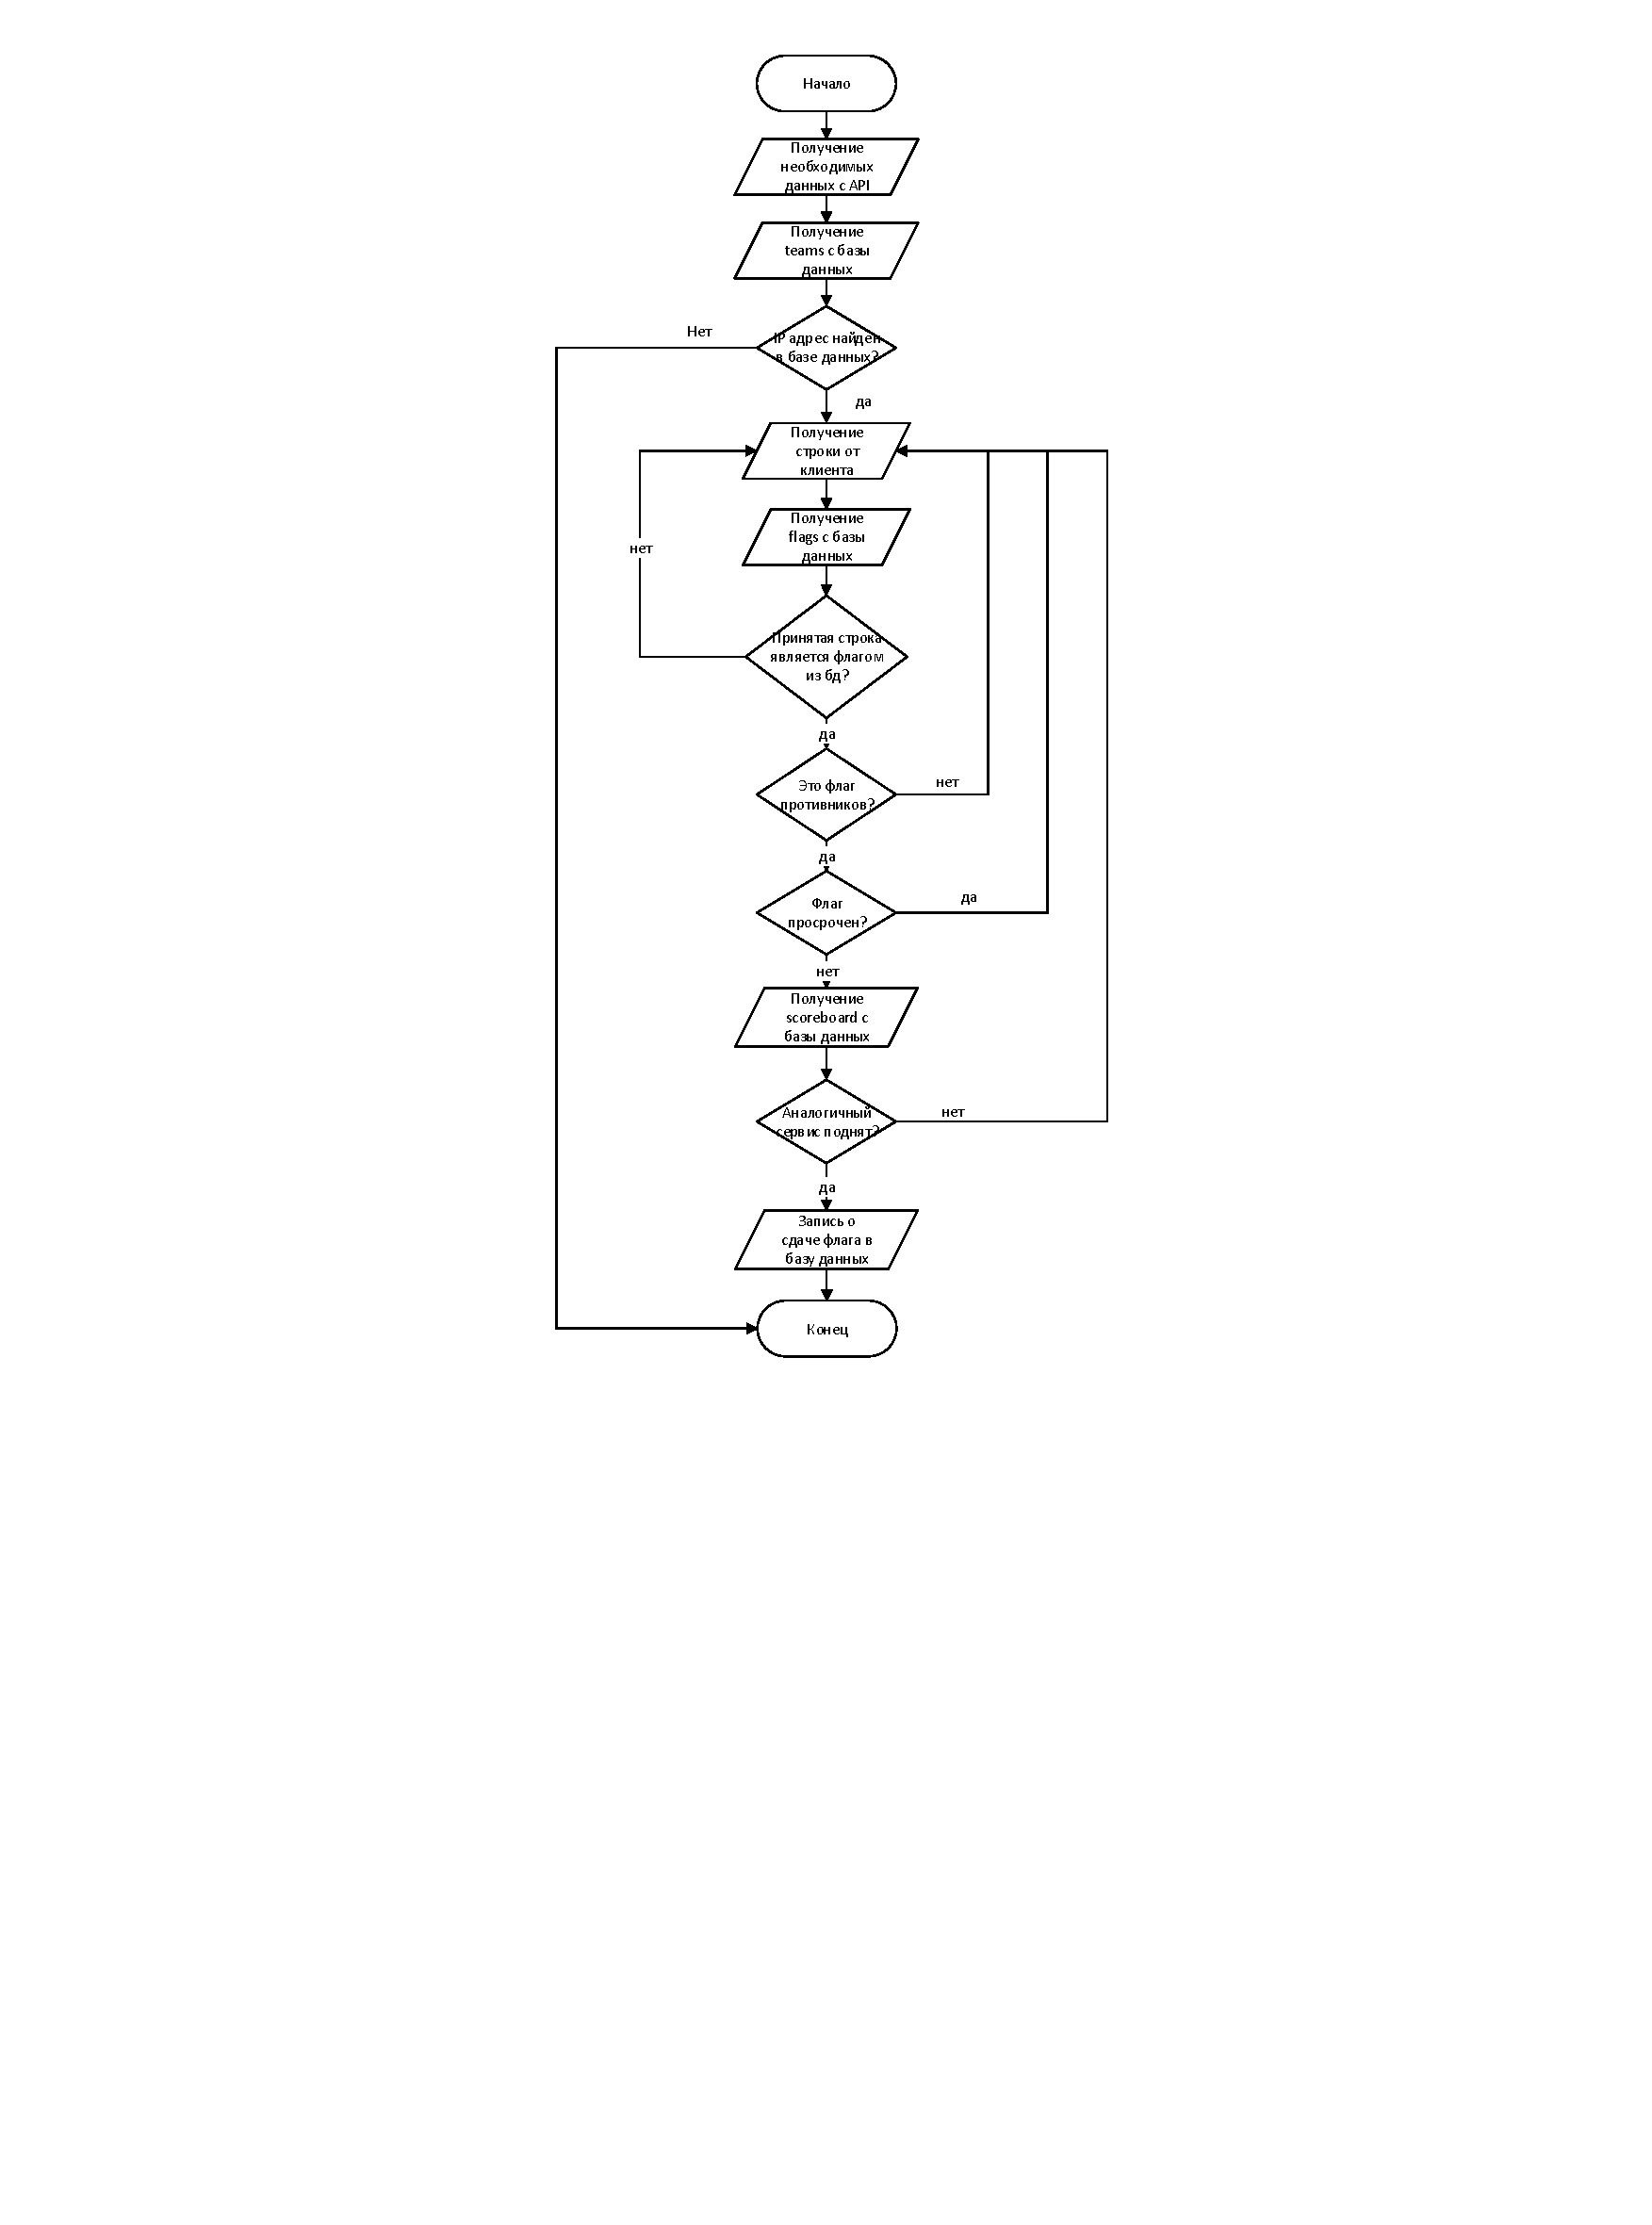
\includegraphics[trim=200 400 200 0, width=0.7\linewidth]{individual_reports/Algoritm.pdf}}
\caption{Алгоритм модуля flags.py}
\end{figure} 

\begin{figure}[h!]
\center{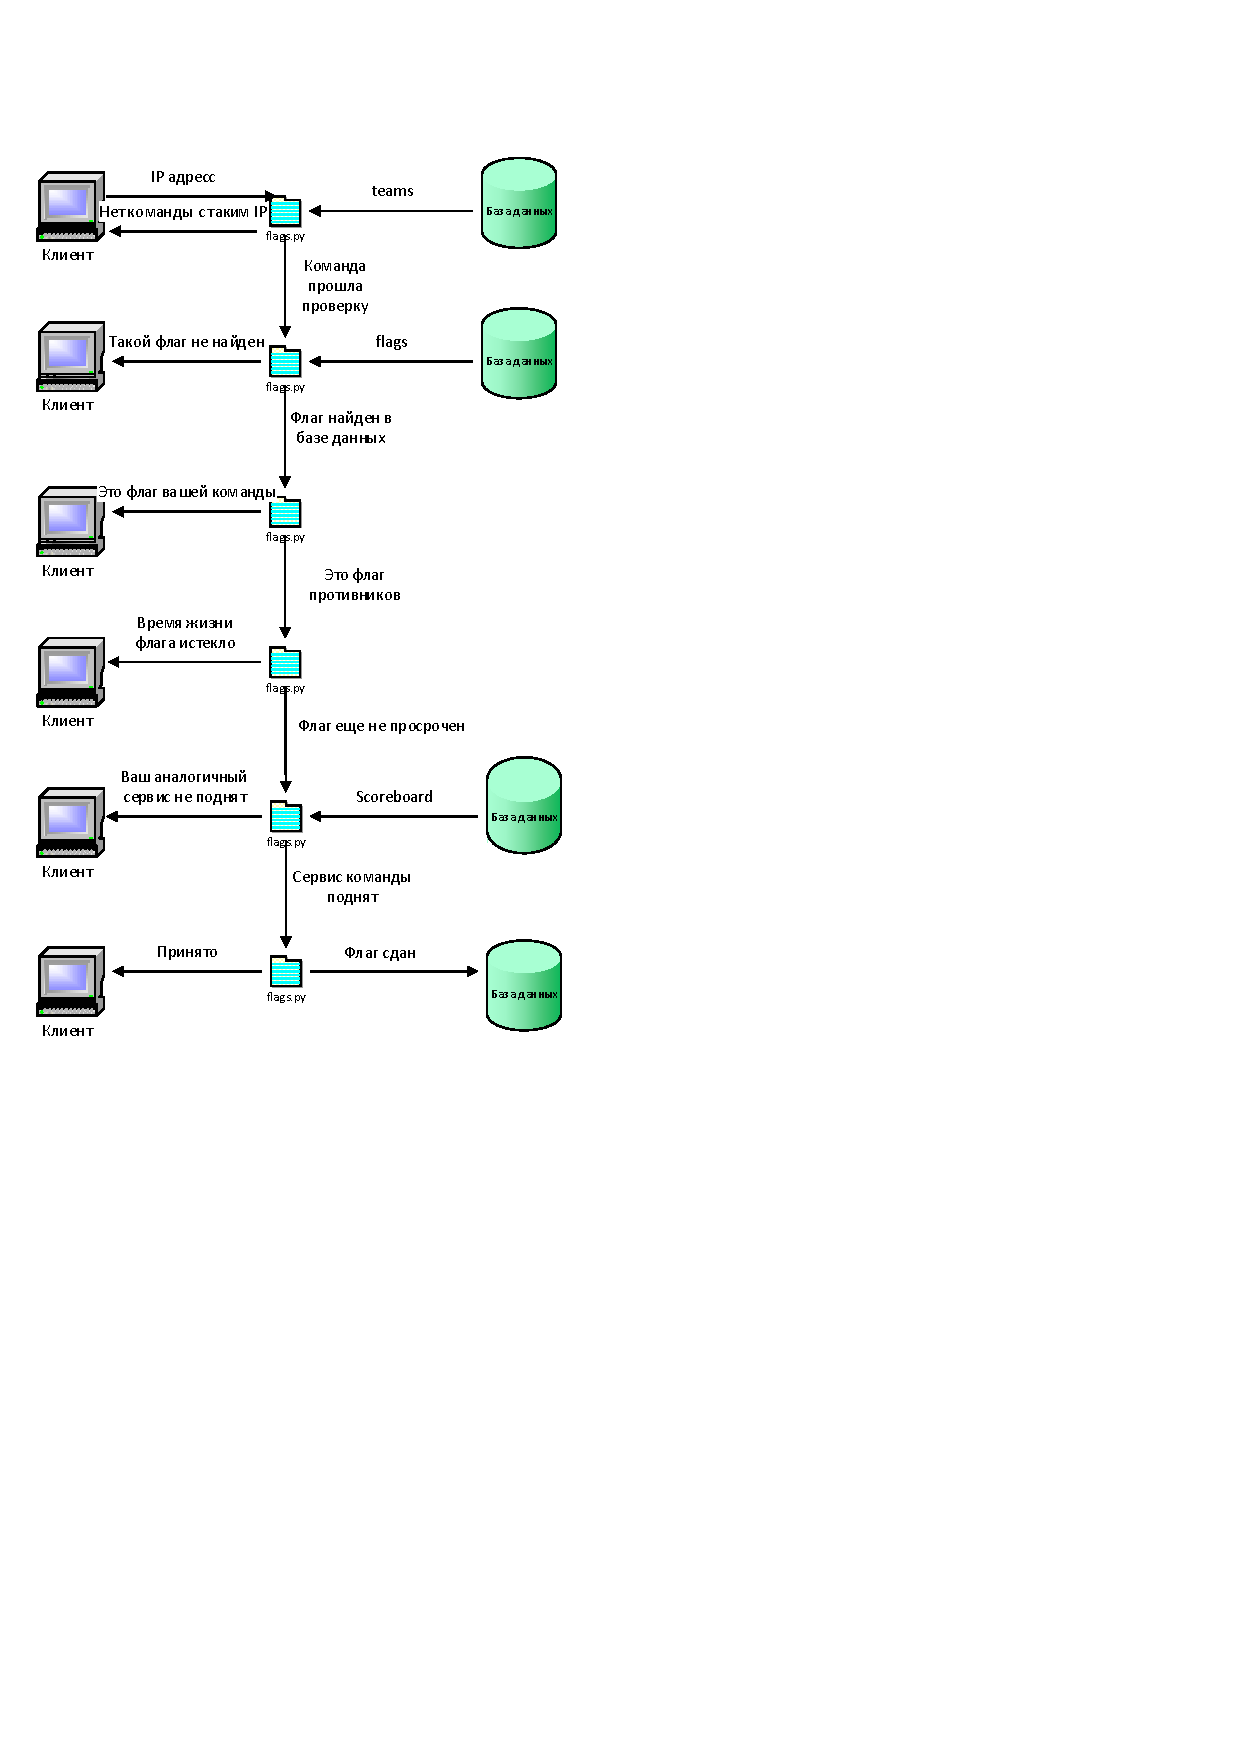
\includegraphics[trim=0 300 300 0, width=0.7\linewidth]{individual_reports/Naglyadno.pdf}}
\caption{Наглядная схема работы flags.py}
\end{figure} 

\clearpage


\subsection{Модуль: таблицы результатов} % - Отчёт scoreboard
Целью работы в текущем семестре стало написание программного модуля, осуществляющего отображения состояния работы сервиса.

\subsubsection{Принцип работы}

Программа реализована с использованием микрофреймворка flask. Программный модуль получает данные из базы данных, выводит результат состояний работы сервисов каждой команды на html страницу.

Ниже представлена схема работы scoreboard.py

\begin{figure}[h!]
\center{\includegraphics[width=0.25\linewidth]{individual_reports/score.png}}
\caption{Cхема работы scoreboard.py}
\end{figure}

\clearpage

\subsection{Модуль: организации работы с сервисами} % - Отчёт round
Основное назначение платформы - общение с сервисами команд-участников посредством отправки и проверки специально сгенерированных флагов на сервере. Предназначение этого модуля - работа с интерфейсом сервисов (чекерами).

\subsubsection{Принцип работы}
Игра делится на раунды, каждый раунд, обычно, длится 1 минуту (настраивается при инициализации). Интерфейс для работы модуля с сервисом называется чекер. За этот период модуль опрашивает с помощью чекеров все сервисы команд-участников. Структура взаимодействия модуля с сервисами представлена на рисунке 5.4.

\begin{figure}[ht!]
\center{\includegraphics[width=1.0\linewidth]{images/module_round_structure.png}}
\caption{Иерархическая структура взаимодействия модуля с сервисами}
\end{figure}

Опрос происходит в три этапа:
\begin{enumerate} 
\item Проверка работоспособности сервиса команды-участника;
\item Отправление флага на сервис; 
\item Проверка того, что флаг сохранен.
\end{enumerate}

На каждом этапе модуль ожидает в ответ один из четырех чисел: 101, 102, 103, 104. Эти числа также называются статусом сервиса команды-участника. Алгоритм работы представлен на рисунке 5.5.

\begin{figure}[ht!]
\center{\includegraphics[width=0.5\linewidth]{images/module_round_schema.png}}
\caption{Схема создания потоков}
\end{figure}


Число 101 соответствует успешной работе сервиса команды-участника. Число 102 означает, что сервис команды работает, но на каком-то этапе отвечает некорректно. Число 103 означает, сервис команды отвечает, но не работает из-за какой-либо ошибки. Число 104 означает, что сервис команды не отвечает на запрос. 

Если на каком-то этапе чекер возвращает число отличное от 101, дальнейшее выполнение программы прекращается, а статус чекера записывается в базу данных.

На 1 этапе каждому чекеру посылается адрес сервера команды-участника. 
На 2 этапе каждому чекеру посылается адрес сервера, идентификатор флага и сам флаг. 
На 3 этапе каждому чекеру посылается адрес сервера, идентификатор флага и сам флаг.

Алгоритм работы представлен на рисунке 5.6.
\begin{figure}[ht!]
\center{\includegraphics[width=0.3\linewidth]{images/module_round_toservice.png}}
\caption{Блок-схема работы с каждым сервисом каждой команды-участника}
\end{figure}


Для увеличения производительности, каждый опрос сервисов команд-участников помещается в новый поток. Это позволяет работать в асинхронном режиме. Поэтому нестабильная работа сервиса команды-участника или ошибка в работе чекера не повлияет на опрос других сервисов. Также каждому потоку задается ограничение по времени работы. Это позволяет своевременно завершать процессы, тем самым уменьшается нагрузка на процессор и на потребление памяти.



\clearpage